% by shahnoor
% shahnoor3pl@gmail.com

\chapter{sheet-17 : Angular Momentum 2: spin 1/2 system}


%%%%% defining graphics path
\ifpdf
\graphicspath{{Chapter17/figs/}}
\else
\graphicspath{{Chapter17/figs/}}
\fi


\setcounter{chapter}{17}
\noindent
\begin{Large}
	{\bf Lecture 17 \newline
		Angular Momentum 2 \newline
		Spin-1/2 System
	}
\end{Large}


\vspace{5 mm}

\section{The Spin Operators and Spin States of a Spin-1/2 Particle}
The electron has an intrinsic angular momentum (i.e., spin angular momentum) in addition to orbital angular momentum. Let the operators corresponding to spin angular momentum of the electron be denoted by
$\hat{S}_x$, $\hat{S}_y$ and $\hat{S}_z$. They satisfy the commutation relations
\be
[\hat{S}_i,\hat{S}_j] = i \hbar\, \epsilon_{ijk}\hat{S}_k \, .
\label{eq:commutation} 
\ee
We can find the common eigenstates of $\hat{S}^2$ and any one of the components, $\hat{S}_z$, say. These eigenstates are denoted by $|s\, m_s\rangle$ where
\be
\hat{S}^2|s\,m_s\rangle = s(s+1)\hbar^2 |s\, m_s\rangle\, ,
\ee
and
\be
\hat{S}_z |s\, m_s\rangle = m_s \hbar |s\, m_s\rangle\, . 
\ee
The spin eigenstates $|s\, m_s\rangle,\; m_s = s,\; s-1,\; \dots ,-s$, can be taken as the basis states in constructing a general spin state.

\paragraph{}
The quantity $s$ is called the spin quantum number (or simply the spin) and the quantity $m_s$ is called the projection quantum number, the projection direction being the $z$-axis. All elementary particles have a definite value for $s$ which is always fixed.
For electrons, as for all leptons and quarks, $s=1/2$. This is why electrons are called a spin-half particles. If $s=1/2$,
the projection quantum number can have only two values, namely $m_s=\pm 1/2$. Therefore, there are only two basis spin states for a spin-1/2 particle. They can be denoted by
\[ |1/2\,\, 1/2\rangle \quad {\rm and} \quad |1/2\,\, -1/2\rangle \, , \]
or by
\[ |S_z\; +\rangle \quad {\rm and} \quad |S_z\; -\rangle \, , \]
or simply
\[ |+\rangle \quad {\rm and} \quad |-\rangle\, . \]
For a spin-1/2 particle, the eigenvalue equations are:
\be
\hat{S}^2|\pm\rangle = \frac{1}{2}\left(\frac{1}{2}+1\right)\hbar^2 |\pm\rangle = \frac{3}{4} \hbar^2 |\pm\rangle
\ee
and
\be
\hat{S}_z|\pm\rangle = \pm \frac{1}{2} \hbar |\pm\rangle\, .
\ee
Using the states $\{ |+\rangle,\; |-\rangle \}$ as the basis set, any general spin state $|\alpha\rangle$ can be expressed as
\be
|\alpha\rangle = |+\rangle \langle +|\alpha\rangle + |-\rangle \langle -|\alpha\rangle\, ,
\ee
or,
\be
|\alpha \rangle= c_+ |+\rangle + c_-|-\rangle \, , 
\ee
where
\be
c_+ = \langle + |\alpha \rangle, \quad {\rm and} \quad c_- = \langle -|\alpha \rangle\, ,
\ee
are the ``components" of $|\alpha \rangle$ along $|+\rangle$ and $|-\rangle$, respectively.
The matrix representation of the general spin state $|\alpha\rangle$ in the basis $\{ |+\rangle,\; |-\rangle \}$ is then
\be
|\alpha\rangle \stackrel{.}{=}\begin{pmatrix} c_+ \\ c_- \end{pmatrix}\equiv \chi\, .
\label{eq:rep}
\ee
The two-component column matrix (Eq. (\ref{eq:rep})) is called the spinor corresponding to the ket $|\alpha\rangle$ and is
denoted by $\chi$. The spinor corresponding to the bra $\langle \alpha|$ is
\be
\langle \alpha | \stackrel{.}{=} \chi^{\dagger} = \begin{pmatrix} c_+^* & c_-^* \end{pmatrix}\, . 
\ee

\paragraph{}
Now we will find the matrix representations of the operators $\hat{S}^2$, $\hat{S}_x$, $\hat{S}_y$ and $\hat{S}_z$ in the
basis $\{ |+\rangle,\,\, |-\rangle\}$. Since the basis set $|+\rangle$ and $|-\rangle$ are eigenstates of
$\hat{S}^2$ and $\hat{S}_z$, it is obvious that in the given basis $\hat{S}^2$ and $\hat{S}_z$ are diagonal. Thus
\be
\hat{S}^2 \stackrel{.}{=} \begin{pmatrix} \langle +|\hat{S}^2|+\rangle & \langle +|\hat{S}^2|-\rangle \\
	\langle -|\hat{S}^2|+\rangle & \langle -|\hat{S}^2|-\rangle
\end{pmatrix}\, ,
\ee
i.e.,
\be
\hat{S}^2 \stackrel{.}{=} \frac{3}{4}\, \hbar^2\begin{pmatrix} 1&0\\0&1\end{pmatrix}\, .
\ee		
Similarly,
\be
\hat{S}_z \stackrel{.}{=} \frac{1}{2}\, \hbar \begin{pmatrix}1&0\\0&-1\end{pmatrix}\, .
\ee
To find the matrix representations of $\hat{S}_x$ and $\hat{S}_y$ in the $\{ |+\rangle,\,|-\rangle \}$ basis, we first introduce two non-Hermitian operators, $\hat{S}_{\pm}$, called raising and lowering operators, and defined by
\be 
\hat{S}_{\pm} = \hat{S}_x \pm i \hat{S}_y\, .
\label{eq:spm}
\ee																			
Using Eq. (\ref{eq:commutation}) we can easily show that
\be
[\hat{S}_z,\hat{S}_{\pm}] = \pm\, \hbar \, \hat{S}_z \, . 
\label{eq:raisinglowering}
\ee  
In other words, Eq. (\ref{eq:raisinglowering}) tells us that the effect of $\hat{S}_{\pm}$ when they act on an eigenstate
of  $\hat{S}_z$ is to give another eigenstate of $\hat{S}_z$ with eigenvalue one unit more ($\hat{S}_{+}$) or
one unit less ($\hat{S}_{-}$). We then have
\be
\hat{S}_+ |+\rangle = 0, \quad {\rm and} \quad \hat{S}_+ |-\rangle = \hbar |+\rangle\, ,
\ee
and
\be
\hat{S}_- |+\rangle = \hbar |-\rangle, \quad {\rm and} \quad \hat{S}_- |-\rangle = 0\, .
\ee
We can now write down the matrix representation of $\hat{S}_+$ and $\hat{S}_-$ in the $\{|+\rangle,\,|-\rangle\}$ basis.
We have
\be
\hat{S}_+ \stackrel{.}{=} \hbar \begin{pmatrix}0&1\\0&0\end{pmatrix}
\ee
\be
\hat{S}_- \stackrel{.}{=} \hbar \begin{pmatrix}0& 0\\1&0\end{pmatrix}\, .
\ee
Next, using Eq. (\ref{eq:spm}) we obtain
\be
\hat{S}_x = \frac{1}{2}\left(\hat{S}_+ + \hat{S}_-\right) \stackrel{.}{=} \frac{1}{2} \hbar\, 
\begin{pmatrix} 0&1\\1&0\end{pmatrix}
\ee
and
\be
\hat{S}_y = \frac{1}{2i}\left(\hat{S}_+ - \hat{S}_-\right) \stackrel{.}{=} \frac{1}{2} \hbar\,
\begin{pmatrix} 0&-i\\i&0\end{pmatrix} \, .
\ee
In summary, we have obtained
\be
\hat{S}_x \stackrel{.}{=} \frac{1}{2}\, \hbar \sigma_x, \quad \hat{S}_y \stackrel{.}{=} \frac{1}{2}\, \hbar \sigma_y, \quad 
\hat{S}_z \stackrel{.}{=} \frac{1}{2}\, \hbar \sigma_z, 
\ee
where $\sigma_x$, $\sigma_y$ and $\sigma_z$ are $2\times 2$ matrices given by
\be
\sigma_x = \begin{pmatrix}0&1\\1&0\end{pmatrix},\quad \sigma_y = \begin{pmatrix}0&-i\\i&0\end{pmatrix},\quad
\sigma_z = \begin{pmatrix}1&0\\0&-1\end{pmatrix}\, .
\ee 
The matrices $\sigma_x$, $\sigma_y$ and $\sigma_z$ are called Pauli matrices.

\subsection{Properties of Pauli Matrices}
In the following we list some properties of Pauli matrices.
\begin{enumerate}
	\item det($\sigma_j$) = -1, \;\;\; j = 1,\;2,\;3.
	\item Tr($\sigma_j$) = 0, \;\;\; j = 1,\;2,\;3.
	\item $\sigma_x^2 = \sigma_y^2 = \sigma_z^2 = I$ where $I$ is the $2\times 2$ unit matrix.
	\item $\sigma_x\sigma_y = - \sigma_y\sigma_x = i\sigma_z$, ($x$, $y$, $z$ cyclic)
	
	\noindent
	It follows that $\{\sigma_x,\sigma_y\}=0$ and $[\sigma_x,\sigma_y]=2i\sigma_z$, i.e., $[ S_x,S_y]=i\hbar S_z$.
	\item Property 3 and 4 are sometime condensed in the form
	\[ \sigma_j\sigma_k = i \epsilon_{jkl}\sigma_l + \delta_{jk}I_{2\times 2}\, , \]
	where $I_{2\times 2}$ is the two-dimensional unit matrix.
	
	\item We can also easily show 
	\[ \sigma_x\sigma_y\sigma_z = i I_{2\times 2}.\]
\end{enumerate}

Finally, we will prove an identity which is very useful. If $\vec{A}$ and $\vec{B}$ are two vectors whose components are numbers
(or operators which commute with all spin operators), then
\be
(\vec{\sigma}.\vec{A})(\vec{\sigma}.\vec{B})= \vec{A}.\vec{B} I_{2\times 2} + i \vec{\sigma}.(\vec{A} \times \vec{B}).
\ee

\noindent 
{\bf Proof:}
\begin{eqnarray*}
	(\vec{\sigma}.\vec{A})(\vec{\sigma}.\vec{B})&=& \sum_{j,k}\sigma_jA_j\sigma_k B_k \\
	&= & \sum_{j,k} A_jB_k\sigma_j\sigma_k \\
	&= & \sum_{j,k} A_jB_k \left[ \sum_l i\epsilon_{jkl}\sigma_l+\delta_{jk}I_{2\times 2}\right] \\
	&=& \sum_l i\sigma_l \left(\sum_{j,k} \epsilon_{jkl}A_jB_k\right) + \sum_j A_jB_j I_{2\times 2}\\
	&=& \sum_l i\sigma_l\left( \vec{A}\times \vec{B}\right)_l + \vec{A}.\vec{B} I_{2\times 2} \\
	& = & i \vec{\sigma}.(\vec{A}\times\vec{B}) + \vec{A}.\vec{B} I_{2\times 2} \;\;\; {\rm (Proved).}
\end{eqnarray*}


\section{Matrix Representations of the Eigenstates of \texorpdfstring{$\hat{S}_x$, $\hat{S}_y$ and $\hat{S}_z$}{PDFstring}}

In the following discussions the eigenstates of $\{ \hat{S}^2, \hat{S}_x\}$, $\{ \hat{S}^2, \hat{S}_y\}$ and
$\{ \hat{S}^2, \hat{S}_z\}$ are denoted by
\[ |S_x,\, \pm\rangle, \;\;\; |S_y,\, \pm\rangle, \;\;\; {\rm and} \;\;\; |S_z,\, \pm\rangle, \;\;\; \]
respectively. We will use the simultaneous eigenkets of $\hat{S}^2$ and $\hat{S}_z$ i.e., the kets $|S_z,\,\, \pm\rangle$ as the basis.
In this basis  the matrix representation of the basis kets themselves are very simple. We have
\be
|S_z,\,+\rangle \stackrel{.}{=} \begin{pmatrix}1\\0 \end{pmatrix}, \quad {\rm and} \quad
|S_z,\,-\rangle \stackrel{.}{=} \begin{pmatrix}0\\1 \end{pmatrix}.
\ee

\paragraph{}
Next, let us find the matrix representations of the states $|S_x,\, \pm\rangle$ in the
$\{ |S_z,\, +\rangle,\, |S_z,\, -\rangle \}$ basis. First, the eigenvalue equations for the states
$|S_x,\, \pm\rangle$ are:
\be
\hat{S}_x |S_x,\, \pm\rangle= \pm \frac{1}{2} \hbar |S_x,\, \pm\rangle \, .
\ee
Let the matrix representation of the state $|S_x,\, +\rangle$ be
\be
|S_x,\, +\rangle \stackrel{.}{=} \begin{pmatrix} x_1\\x_2\end{pmatrix} \, .
\ee
Therefore, the eigenvalue equation of $|S_x,\, +\rangle$ in matrix form can be written as
\be
\frac{1}{2} \hbar\sigma_x \begin{pmatrix} x_1\\x_2\end{pmatrix} = \frac{1}{2}\hbar \begin{pmatrix} x_1\\x_2\end{pmatrix}\,,
\ee
or,
\[ \sigma_x \begin{pmatrix} x_1\\x_2\end{pmatrix} = \begin{pmatrix} x_1\\x_2\end{pmatrix}\, , \]
or,
\[ \begin{pmatrix}0&1\\1&0\end{pmatrix} \begin{pmatrix} x_1\\x_2\end{pmatrix} = \begin{pmatrix} x_1\\x_2\end{pmatrix} \]
i.e.,
\[  \begin{pmatrix} x_2\\x_1\end{pmatrix} = \begin{pmatrix} x_1\\x_2\end{pmatrix}. \]
This equation tells us that $x_1=x_2$. Therefore, the matrix representation of the state
$|S_x,\,+\rangle$ is of the form
\[ |S_x,\,+\rangle \stackrel{.}{=} \begin{pmatrix} x_1\\x_1\end{pmatrix} \, . \]
Normalizing, we have
\be
|S_x,\,+\rangle \stackrel{.}{=} \frac{1}{\sqrt{2}}\, \begin{pmatrix}1\\1\end{pmatrix} \, . 
\ee
Similarly, we can find the matrix representation for the state $|S_x,\,-\rangle$:
\be
|S_x,\,-\rangle \stackrel{.}{=} \frac{1}{\sqrt{2}}\, \begin{pmatrix}1\\-1\end{pmatrix} \, . 
\ee

\paragraph{}
Following the same procedure, we find the matrix representations of the states $|S_y,\, +\rangle$ and
$|S_y,\, -\rangle$  in the $\{ |S_z,\, +\rangle,\, |S_z,\, -\rangle\}$ basis. We find
\be
|S_y,\, +\rangle \stackrel{.}{=} \frac{1}{\sqrt{2}} \begin{pmatrix} 1\\i\end{pmatrix}\, , 
\ee
and
\be
|S_y,\, -\rangle \stackrel{.}{=} \frac{1}{\sqrt{2}} \begin{pmatrix} 1\\-i\end{pmatrix}\, .
\ee


\subsubsection{Summary}
In summary, we have obtained the following representations in the $\{ |S_z,\, +\rangle,\, |S_z,\, -\rangle\}$ basis:
\be
|S_z,\,+\rangle \stackrel{.}{=} \begin{pmatrix}1\\0\end{pmatrix}, \quad 
|S_z,\,-\rangle \stackrel{.}{=} \begin{pmatrix}0\\1\end{pmatrix}\,.
\ee
Also
\be
|S_x,\,+\rangle \stackrel{.}{=} \frac{1}{\sqrt{2}}\, \begin{pmatrix}1\\1\end{pmatrix} =
\frac{1}{\sqrt{2}}\, \begin{pmatrix}1\\0\end{pmatrix} + \frac{1}{\sqrt{2}}\, \begin{pmatrix}0\\1\end{pmatrix}
\ee
and
\be
|S_x,\,-\rangle \stackrel{.}{=} \frac{1}{\sqrt{2}}\, \begin{pmatrix}1\\-1\end{pmatrix} =
\frac{1}{\sqrt{2}}\, \begin{pmatrix}1\\0\end{pmatrix} - \frac{1}{\sqrt{2}}\, \begin{pmatrix}0\\1\end{pmatrix}.
\ee
In terms of the abstract vectors we can write
\begin{eqnarray}
|S_x,\, +\rangle &=& \frac{1}{\sqrt{2}}\, |S_z,\, +\rangle + \frac{1}{\sqrt{2}}\, |S_z,\, -\rangle \label{eq:sxplus}\\
|S_x,\, -\rangle &=& \frac{1}{\sqrt{2}}\, |S_z,\, +\rangle - \frac{1}{\sqrt{2}}\, |S_z,\, -\rangle \label{eq:sxminus}
\end{eqnarray}
Next,
\be
|S_y,\,+\rangle \stackrel{.}{=} \frac{1}{\sqrt{2}}\, \begin{pmatrix}1\\i\end{pmatrix} =
\frac{1}{\sqrt{2}}\, \begin{pmatrix}1\\0\end{pmatrix} + \frac{i}{\sqrt{2}}\, \begin{pmatrix}0\\1\end{pmatrix}
\ee
and
\be
|S_y,\,-\rangle \stackrel{.}{=} \frac{1}{\sqrt{2}}\, \begin{pmatrix}1\\-i\end{pmatrix} =
\frac{1}{\sqrt{2}}\, \begin{pmatrix}1\\0\end{pmatrix} - \frac{i}{\sqrt{2}}\, \begin{pmatrix}0\\1\end{pmatrix}.
\ee
In terms of the abstract vectors we can write
\begin{eqnarray}
|S_y,\, +\rangle &=& \frac{1}{\sqrt{2}}\, |S_z,\, +\rangle + \frac{i}{\sqrt{2}}\, |S_z,\, -\rangle \label{eq:syplus}\\
|S_y,\, -\rangle &=& \frac{1}{\sqrt{2}}\, |S_z,\, +\rangle - \frac{i}{\sqrt{2}}\, |S_z,\, -\rangle \label{eq:syminus}
\end{eqnarray}

\subsubsection{Spin Probabilities}
Using equations (\ref{eq:sxplus}), (\ref{eq:sxminus}), (\ref{eq:syplus}) and (\ref{eq:syminus}) we can work out the probabilities for finding specific spin values in measurements of spin. For example, suppose that the spin state of the electron is
$|S_z,\, +\rangle$. If we measure the $x$-component of the electron's spin, what is the probability that the measurement will yield the value $\frac{1}{2}\hbar$? Using the postulates of quantum mechanics, we obtain
\be
P\left(S_x=\frac{1}{2}\hbar\right) = \left| \langle S_x,\, +|S_z,\,+\rangle\right|^2 = \left(\frac{1}{\sqrt{2}}\right)^2 = \frac{1}{2}.
\ee
Similarly, the probability that the measurement of $S_x$ gives $-\frac{1}{2}\hbar$ is
\be
P\left(S_x=-\frac{1}{2}\hbar\right) = \left| \langle S_x,\, -|S_z,\,+\rangle\right|^2 = \left(\frac{1}{\sqrt{2}}\right)^2 = \frac{1}{2}.
\ee
This result is dramatically illustrated in an experiment with two Stern-Gerlach arrangements as described below.


\newpage

\subsubsection{Stern-Gerlach Apparatus for Electron Spin}

\begin{figure}[ht]
	\centering
	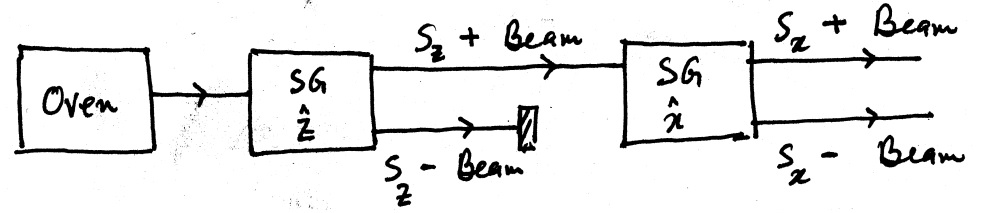
\includegraphics[height=0.32\linewidth, width=\linewidth]{sg.jpg}
	\caption{Stern-Gerlach apparatus for electron spin. }
	\label{sg}
\end{figure}

Silver atoms from an oven are made to pass through a Stern-Gerlach arrangement in which the inhomogeneity in the magnetic field is 
along the $z$-axis ((SG $\hat{z}$). The beam divides into two components of equal intensity. In one of the beams all the silver atoms are in the $|S_z,\, +\rangle$ state and in the other beam all of the atoms are in the $|S_z,\,-\rangle$ state. 

\paragraph{}
Now, suppose that the $|S_z,\,-\rangle$ beam is blocked. The other beam is allowed to pass through a second Stern-Gerlach apparatus in which the inhomogeneity of the magnetic field is along the $x$-axis (SG $\hat{x}$). We find that the $|S_z,\,+\rangle$
beam which entered the SG $\hat{x}$ apparatus divides into two beams of equal intensities. This shows that if electrons are in  the state  $|S_z,\,+ \rangle$, then there is an equal probability that a
measurement of $S_x$ will give $\frac{1}{2}\hbar$ or $-\frac{1}{2}\hbar$.

\newpage

\section{Eigenvalues and Eigenvectors of \texorpdfstring{$\hat{\vec{S}}. \hat{n}$}{PDFstring} }
So far we have found the eigenvalues and the eigenvectors of the operators $\hat{S}_x$, $\hat{S}_y$ and
$\hat{S}_z$. We shall now find an expression for the eigenvectors of the operator $\hat{\vec{S}}.\hat{n}$ in the 
$|S_z,\, \pm\rangle$ basis. Here $\hat{n}$ is an arbitrary direction characterized by the polar angle $\theta$ and the azimuthal angle $\phi$ (figure below).
\begin{figure}[h]
	\centering
	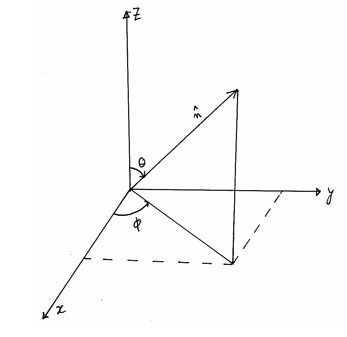
\includegraphics[scale=0.9]{direction.jpg}
	\vspace{-0.5 cm}
	\caption{A direction $\hat{n}$ in space is characterized by two angles in the spherical coordinate system, namely, the polar angle
		$\theta$ and the azimuthal angle $\phi$. }
	\label{fig:direction}
\end{figure}

The operator $\hat{\vec{S}}.\hat{n}$ represents the component of the spin angular momentum along $\hat{n}$. We can write $\hat{n}$ as
\begin{eqnarray}
\hat{n} & = & \hat{i}\,n_x + \hat{j}\, n_y + \hat{k}\, n_z \nonumber \\
& = & \hat{i}\, \sin\theta\, \cos \phi + \hat{j}\, \sin\theta\, \sin \phi + \hat{k}\, \cos\theta \, . 
\label{eq:nhat}
\end{eqnarray}

\paragraph{}
Now, the matrix representation of the operator $\hat{\vec{S}}.\hat{n}$ in the $|S_z,\,\pm\rangle$ basis is 
$\frac{1}{2} \hbar\, \vec{\sigma}.\hat{n}$. Therefore,

\be
\left( \hat{\vec{S}}.\hat{n}\right)^2 \stackrel{.}{=} \left(\frac{1}{2}\hbar\, \vec{\sigma}.\hat{n} \right)^2
= \frac{\hbar^2}{4} \left( \vec{\sigma}.\hat{n}\right)^2 = \frac{\hbar^2}{4} I\, .
\ee
Hence, the eigenvalues of $\hat{\vec{S}}.\hat{n}$ are $\pm \, \hbar/2$.

\paragraph{}
Let us now find the eigenvectors of $\hat{\vec{S}}.\hat{n}$ with eigenvalues $+\frac{1}{2}\, \hbar$. First, we write the eigenvalue equation:
\be 
\hat{\vec{S}}.\hat{n}\, |S_n,\, +\rangle = \frac{1}{2} \, \hbar \, |S_n,\, +\rangle\, . 
\label{eq:eigenvalue1}
\ee
In the $\{ |S_z,\,+\rangle,\, |S_z,\,-\rangle\}$ basis, the matrix representation of the operator $\hat{\vec{S}}.\hat{n}$ is
\begin{eqnarray}
\hat{\vec{S}}.\hat{n} &\stackrel{.}{=}& \frac{1}{2}\, \hbar\, \vec{\sigma}.\hat{n} \nonumber \\
& = & \frac{1}{2}\, \hbar\, \sigma_x \sin\theta\, \cos \phi + \frac{1}{2}\, \hbar\, \sigma_y \sin\theta\, \sin \phi
+ \frac{1}{2}\, \hbar\, \sigma_z \cos\theta \nonumber \\
& = & \frac{1}{2}\, \hbar\, \begin{pmatrix} \cos \theta & \sin\theta e^{-i\phi} \\
\sin\theta\, e^{i\phi}& -\cos\theta
\end{pmatrix}.
\end{eqnarray}		
Let the matrix representation of $|S_n,\,+\rangle$ in the same basis be
\be
|S_n,\,+\rangle \stackrel{.}{=} \begin{pmatrix}x_1\\x_2\end{pmatrix},
\ee
i.e.,
\be
\langle S_z,\,+|S_n,\,+\rangle = x_1, \quad {\rm and} \quad			
\langle S_z,\,-|S_n,\,+\rangle = x_2																	.
\ee
Therefore, the matrix representation of the eigenvalue equation (\ref{eq:eigenvalue1}) is
\[ \frac{1}{2}\, \hbar\, \begin{pmatrix} \cos \theta & \sin\theta e^{-i\phi} \\
\sin\theta\, e^{i\phi}& -\cos\theta
\end{pmatrix}\begin{pmatrix}x_1\\x_2\end{pmatrix} = 
\frac{1}{2}\,\hbar\, \begin{pmatrix}x_1\\x_2\end{pmatrix}. \]
Canceling the factor $\frac{1}{2}\, \hbar$ from both sides we get
\[ \begin{pmatrix} \cos \theta & \sin\theta e^{-i\phi} \\
\sin\theta\, e^{i\phi}& -\cos\theta
\end{pmatrix}\begin{pmatrix}x_1\\x_2\end{pmatrix} = 
\begin{pmatrix}x_1\\x_2\end{pmatrix}, \]
or,
\[ \begin{pmatrix}\cos\theta\,x_1+\sin\theta\,e^{-i\phi}\,x_2\\
\sin\theta\,e^{i\phi}\,x_1-\cos\theta\,x_2 \end{pmatrix} = 
\begin{pmatrix}x_1\\x_2 \end{pmatrix}. \]
Therefore,
\[ \cos \theta\, x_1 + \sin\theta\, e^{-i\phi}\, x_2 = x_1 \, , \]
i.e.,
\[ (1-\cos\theta)x_1=\sin\theta\, e^{-i\phi}\, x_2\, ,\]
or,
\[ 2\sin^2 \frac{\theta}{2}\, x_1 = 2\sin \frac{\theta}{2}\,\cos \frac{\theta}{2}\, e^{-i\phi}\,x_2\, .\]
From the above equation we get
\be
\frac{x_1}{x_2}= \frac{e^{-i\phi/2}\cos \theta/2}{e^{i\phi/2}\sin \theta/2}\, .
\ee
Hence, the normalized matrix representation for the state $|S_n,\,+\rangle$ is
\begin{eqnarray}
|S_n,\,+\rangle &\stackrel{.}{=}& \begin{pmatrix}e^{-i\phi/2}\cos \theta/2\\ e^{i\phi/2}\sin\theta/2\end{pmatrix} \nonumber \\
& = & e^{-i\phi/2}\, \cos \theta/2 \begin{pmatrix}1\\0\end{pmatrix} + e^{i\phi/2}\, \sin \theta/2\begin{pmatrix}0\\1\end{pmatrix}.
\end{eqnarray}
The above equation can be written in terms of the abstract vectors in the Hilbert space as
\be
\boxed{
	|S_n,\,+\rangle = e^{-i\phi/2}\, \cos \frac{\theta}{2}\, |S_z,\, +\rangle + e^{i\phi/2}\, \sin \frac{\theta}{2}\,|S_z,\,-\rangle\, .
}
\ee


\paragraph{}
Proceeding in a similar fashion, we can find the matrix representation of $|S_n,\,-\rangle$ in the
$\{ |S_z,\,+\rangle,\, |S_z,\,-\rangle\}$ basis. We get 
\be
|S_n,\,-\rangle \stackrel{.}{=} \begin{pmatrix} -e^{-i\phi/2}\sin \theta/2\\e^{i\phi/2}\cos \theta/2\end{pmatrix},
\ee
i.e.,
\be
\boxed{
	|S_n,\,-\rangle = -e^{-i\phi/2}\sin \theta/2\, |S_z,\,+\rangle   +  e^{i\phi/2}\cos \theta/2\, |S_z,\,-\rangle\, .
}
\ee




% New section
\section{Non-relativistic Description of a Spin-1/2 Particle}
\subsection{Basis Vectors}
So far we have considered quantum mechanical description of a system having spatial degrees of freedom or spin degrees
of freedom only. But a system, an electron say, can have both spatial and spin degrees of freedom. How is our fromulation
to be generalized to include both these degrees of freedom?

\paragraph{}
We note that to describe a quantum system we first need to establish a basis of states. The basis set could be written in many different ways. To set up a basis, we need a complete set of cummutating observables (CSCO) of the system and the simultaneous 
eigenstates of these observables could serve as a basis.

\paragraph{}
For a point particle with spin, the CSCO can be chosen in various ways as shown below:
\[ \{\hat{\vec{R}}, \hat{S}^2, \hat{S}_z\} \]
\[ \{\hat{\vec{P}}, \hat{S}^2, \hat{S}_z\} \]
\[ \{\hat{H}, \hat{L}^2, \hat{L}_z,\hat{S}^2, \hat{S}_z\}. \]
We shall use the first set of CSCO. Let $|\vec{r}\rangle$ and $|\epsilon\rangle$ be the eigenkets of $\hat{\vec{R}}$ and
$\{ \hat{S}^2,\, \hat{S}_z\}$, respectively, i.e.,
\begin{eqnarray}
\hat{\vec{R}}\, |\vec{r}\rangle &=& \vec{r}\, |\vec{r}\rangle \\
\hat{S}^2\, |\epsilon\rangle & =& s(s+1)\hbar^2\, |\epsilon\rangle \\
\hat{S}_z\, |\epsilon\rangle & =& \frac{1}{2}\, \hbar\,\epsilon |\epsilon\rangle \quad (\epsilon = 2 m_s).
\end{eqnarray}
For a spin-1/2 particle, $s=1/2$, therefore, there are only two possible linearly independent basis states with
$\epsilon=1$ and $\epsilon=-1$, corresponding to the $z$-component of spin being equal to $\frac{1}{2}\, \hbar$
and $-\frac{1}{2}\, \hbar$, respectively. In other words
\be
\hat{S}^2 |\pm\rangle = \frac{3}{4}\, \hbar^2\, |\pm\rangle \, , 
\ee
\be
\hat{S}_z |\pm\rangle = \pm \frac{1}{2}\, \hbar\, |\pm\rangle \, ,
\ee
where we have labelled the states as $|+\rangle \equiv |\epsilon = 1\rangle$ and $|-\rangle \equiv |\epsilon = -1\rangle$.
Now, since the space and spin degrees of freedom are independent, we have
\be
[\hat{\vec{R}},\hat{\vec{S}}]=0\, .
\ee
The simultaneous eigenkets $|\vec{r},\epsilon\rangle$ of the CSCO $\{\hat{\vec{R}}, \hat{S}^2, \hat{S}_z\}$
can then be written as a product
\be
|\vec{r}, \epsilon\rangle = |\vec{r}\,\rangle |\epsilon\rangle\, .
\label{eq:tensorproduct}
\ee
That is, the ket space formed by the eigenkets of $\{\hat{\vec{R}}, \hat{S}^2, \hat{S}_z\}$ is a tensor product of the ket space
spanned by the eigenkets $|\vec{r}\,\rangle$ of $\hat{\vec{R}}$ and the eigenkets $|\epsilon\rangle$ of
$\{\hat{S}^2, \hat{S}_z\}$. Thus
\be
H= H_{\vec{r}} \otimes H_s \, .
\ee
The orthogonality and completeness conditions of the basis kets $|\vec{r},\epsilon\rangle$ are
\be
\langle \vec{r}^{\,\,\prime}\, \epsilon^{\prime}|\vec{r}\, \epsilon \rangle = \delta(\vec{r}\, - \vec{r}^{\,\,\prime}\,)
\delta_{\epsilon\epsilon^{\prime}}
\ee
and
\be
\sum_{\epsilon}\int d^3r\, |\vec{r}\,\epsilon\rangle\langle \vec{r}\,\epsilon| = \hat{I}\, .
\label{eq:completeness1}
\ee
For spin-1/2 particles, $\epsilon=\pm$, and the completeness condition, i.e., Eq. (\ref{eq:completeness1}) can be written more explicitly as
\be
\int d^3r\, |\vec{r}\, +\rangle\langle \vec{r}\,+| + \int d^3r\, |\vec{r}\, -\rangle\langle \vec{r}\, -| = \hat{I}\, .
\ee


\subsection{State Vector}

Any general state $|\psi\rangle$ of the particle can be expanded as a linear combination of the basis kets
$|\vec{r}\, \epsilon\rangle$:
\begin{eqnarray}
|\psi\rangle &= & \sum_{\epsilon} \int d^3r\, |\vec{r}\, \epsilon\rangle \langle \vec{r}\, \epsilon|\psi\rangle \nonumber \\
& = & \sum_{\epsilon}\int d^3r\, |\vec{r}\, \epsilon\rangle \, \psi_{\epsilon}(\vec{r}\,)
\end{eqnarray}
where we have defined
\be
\psi_{\epsilon}(\vec{r}\,) = \langle \vec{r}\, \epsilon|\psi\rangle\, .
\ee
The numbers $\psi_{\epsilon}(\vec{r}\,)$ which depend on three continuous indices (i.e., $x$, $y$ and $z$) and on one
discrete index $\epsilon$ ( $+$ or $-$ for a spin-1/2 particle), can be considered as the `coordinates' of the state
$|\psi\rangle$ in the $|\vec{r}\, \epsilon\rangle$ basis. Thus, in order to characterize the state of a spin-1/2 particle
completely, we have to specify \underline{two} functions of the space variables $x$, $y$ and $z$:
\be
\psi_+(\vec{r}\,) \equiv \langle \vec{r},\, +|\psi\rangle, \quad {\rm and} \quad
\psi_-(\vec{r}\,) \equiv \langle \vec{r},\, -|\psi\rangle.
\ee
These two functions are often written in the form of a two-component column matrix, called a spinor, which we shall
denote as $[\psi](\vec r\,)$, i.e.,
\be 
[\psi](\vec{r}\,) = \begin{pmatrix}\psi_+(\vec{r}\,)\\\psi_-(\vec{r}\,)\end{pmatrix}.
\ee
The bra $\langle \psi|$ associated with the ket $|\psi\rangle$ is given by
\begin{eqnarray}
\langle \psi| &=& \sum_{\epsilon} \int d^3r\, \langle \psi|\vec{r}\, \epsilon\rangle \langle \vec{r}\, \epsilon| \nonumber \\
& = & \sum_{\epsilon} \int d^3r\, \psi_{\epsilon}^*(\vec{r}\,)\langle \vec{r}\,\epsilon|\, .
\end{eqnarray}
The bra $\langle \psi|$ is thus represented by two functions $\psi_+^*(\vec{r}\,)$ and $\psi_-^*(\vec{r}\,)$, written
as a row matrix which is the adjoint of $[\psi](\vec{r}\,)$. Thus
\be
\langle \psi| \stackrel{.}{=} [\psi]^{\dagger}(\vec{r}\,) = \begin{pmatrix} \psi_+^*(\vec{r}\,)&\psi_-^*(\vec{r}\,)\end{pmatrix}.
\ee
With this notation, the scalar product of two vectors $|\psi\rangle$ and $|\phi\rangle$ can be written as
\begin{eqnarray}
\langle \psi|\phi\rangle &=& \sum_{\epsilon}\int d^3r\, \langle\psi|\vec{r}\, \epsilon\rangle\langle\vec{r}\,\epsilon|\phi\rangle \nonumber \\
& = & \sum_{\epsilon}\int d^3r\,\psi_{\epsilon}^*(\vec{r}\,)\phi_{\epsilon}(\vec{r}\,) \nonumber \\
& = & \int d^3r\, \begin{pmatrix}\psi_+^*(\vec{r}\,)&\psi_-^*(\vec{r}\,)\end{pmatrix}
\begin{pmatrix}\phi_+(\vec{r}\,)\\\phi_-(\vec{r}\,)\end{pmatrix} \nonumber \\
&= & \int d^3r\, [\psi]^{\dagger}(\vec{r}\,)	[\phi](\vec{r}\,).
\end{eqnarray}			
In particular, the normalization of the state vector $|\psi\rangle$ is expressed as
\begin{eqnarray}
\langle\psi|\psi\rangle &=& \int d^3r\, [\psi]^{\dagger}(\vec{r}\,)[\psi](\vec{r}\,) \nonumber \\
& = & \int d^3r\, \left[ |\psi_+(\vec{r}\,)|^2 + |\psi_-(\vec{r}\,)|^2\right] =1.
\end{eqnarray}		

\subsubsection{Probabilistic Interpretation of the wavefunctions $\psi_{\pm}(\vec{r}\,)$}
We have have the following interpretation for the wave functions:

\begin{itemize}
	\item 
	$|\psi_+(\vec{r}\,)|^2\, d^3r $ = 
	probability that the electron is found in a small volume $d^3r$ around $\vec{r}$ with the $z$-component of the spin 
	$\frac{1}{2}\,\hbar$. A similar interpretation holds for $|\psi_-(\vec{r}\,)|^2\, d^3r$.
\end{itemize}
If we integrate $|\psi_+(\vec{r}\,)|^2\, d^3r $ over $\vec{r}$ we get
\begin{itemize}
	\item
	$\int |\psi_+(\vec{r}\,)|^2\, d^3r$  =
	probability that the $z$-component of the electron's spin is $\frac{1}{2}\, \hbar$ irrespective of its position. Similarly
	\item
	$\int |\psi_-(\vec{r}\,)|^2\, d^3r$  =
	probability that the $z$-component of the electron's spin is $-\frac{1}{2}\, \hbar$ irrespective of its position. 
\end{itemize}

As a final comment, we note that the basis vectors for a spin-1/2 particle are tensors products of a ket belonging
to $H_{\vec{r}}$ and a ket belonging to $H_s$ (Eq. \ref{eq:tensorproduct}). However, the state vector may or may not be a
tensor product of a vector in $H_{\vec{r}}$ and a vector in $H_s$. Only in the special case when the Hamiltonian is spin-independent
the state vector $|\psi\rangle$ is of this type, i.e.,
\[ |\psi\rangle = |\phi\rangle |\alpha\rangle \, , \]
where
\[ |\phi\rangle \in H_{\vec{r}}, \quad {\rm and} \quad |\alpha\rangle \in H_s\, .\]
In this case we have
\begin{eqnarray}
\psi_{\epsilon}(\vec{r}\,) &=& \langle \vec{r}\,\epsilon|\psi\rangle \nonumber \\
&=& \left(  \langle\vec{r}\,| \langle \epsilon\,|  \right) \left( |\phi\rangle |\alpha\rangle \right) \nonumber \\
&=& \langle\vec{r}\,|\phi\rangle\langle \epsilon |\alpha\rangle \nonumber \\
&=& \phi(\vec{r}\,)c_{\epsilon},
\end{eqnarray}
where
\be
c_{\epsilon}=\langle\epsilon|\alpha\rangle\ .
\ee 


\paragraph{}
For a spin-1/2 particles $\epsilon = \pm$, and in the special case of spin-independent Hamiltonian we have
\[ \psi_+(\vec{r}\,) = \phi(\vec{r}\,)c_+ \]
and
\[ \psi_-(\vec{r}\,) = \phi(\vec{r}\,)c_-\,.\]
Therefore, the spinor $[\psi](\vec{r}\,)$ is
\be
[\psi](\vec{r}\,) = \begin{pmatrix}\psi_+(\vec{r}\,)\\\psi_-(\vec{r}\,)\end{pmatrix}
= \phi(\vec{r}\,)\begin{pmatrix}c_+\\c_-\end{pmatrix}.
\ee
The square of the norm of $|\psi\rangle$ is then given by
\be
\langle\psi|\psi\rangle= \langle\phi|\phi\rangle \langle \chi|\chi\rangle = (|c_+|^2+|c_-|^2)\int d^3r\, |\phi(\vec{r}\,)|^2\, .
\ee

\section{Electron in an External Magnetic Field. Pauli Equation}
Suppose that an electron is placed in an external time-independent magnetic field $\vec{B}$. The magnetic moment operator of the
electron is 
\be
\hat{\vec{\mu}} =  = \hat{\vec{\mu}}_{{\rm orbit}} + \hat{\vec{\mu}}_{{\rm spin}}\, ,
\ee
where
\be
\hat{\vec{\mu}}_{{\rm orbit}} = \frac{q_e}{2m_e} \hat{\vec{L}} 
\ee
and
\be
\hat{\vec{\mu}}_{{\rm spin}} =g_s \frac{q_e}{2m_e} \hat{\vec{S}}\, .
\ee
Here $q_e$ is the charge of the electron, i.e., $q_e=-e$ with $e=1.6 \times 10^{-19}$ C, and $g_s$ is the spin
gyromagnetic ratio. From Dirac theory we have $g_s=2$ for electrons. The total magnetic moment of the electron is then
\be
\hat{\vec{\mu}} = \frac{q_e}{2m_e} (\hat{\vec{L}} + 2 \hat{\vec{S}} )\, .
\ee 
In the spin space of the electron, we can express $\hat{\vec{\mu}}$ as a $2\times 2$ matrix:
\be
\hat{\vec{\mu}} = \frac{q_e}{2m_e} (\hat{\vec{L}}\; \hat{1}_{2\times 2} + \hbar \vec{\sigma} )
\ee
where we have used the matrix representation of the spin operator of a spin-1/2 particle, i.e.,
\be
\hat{\vec{S}} \stackrel {.}{=} \frac{1}{2}\,\hbar\, \vec{\sigma}\, ,
\ee
and $\hat{1}_{2\times 2}$ is a unit $2\times 2$ matrix.

\paragraph{}
Now, the interaction energy of the electron with the external magnetic field is
\begin{eqnarray}
V &=& -\hat{\vec{\mu}}.\vec{B} \nonumber \\
& = & \mu_{B}\left( \frac{\hat{\vec{L}}}{\hbar}\, \hat{1}_{2\times 2} + \vec{\sigma} \right).\vec{B} \, ,
\end{eqnarray}
where
\be
\mu_B = \frac{|q_e|\hbar}{2m_e} = \frac{e\hbar}{2m_e}\, 
\ee
is the Bohr magneton. Here $e$ is the magnitude of charge of the electron, hence $e$ is a positive number,
$e=1.6\times 10^{-19}$ C. The Hamiltonian operator of the electron is then
\be
\hat{H} = \left( \frac{\hat{\vec{p}}^{\,2}}{2m_e} + V(\hat{\vec{r}}\,) \right ) I_{2\times 2} + \mu_{B}\left( \frac{\hat{\vec{L}}}{\hbar}\, \hat{1}_{2\times 2} + \vec{\sigma} \right).\vec{B}\, ,
\ee
where $V(\hat{\vec{r}}\,)$ is the potential energy of the electron's interaction with other fields, for example, the Coulomb field of the nucleus if the electron is bound in an atomic orbit. The Schr\"{o}dinger equation for the electron is then
\be
i\hbar \frac{\partial}{\partial t}\, |\psi\rangle = \hat{H} |\psi\rangle\,,
\ee
or, in terms of the components of $|\psi\rangle$
\begin{multline}
i \hbar\, \frac{\partial}{\partial t}\, \begin{pmatrix}\psi_+(\vec{r}\, , t)\\ \psi_+(\vec{r}\, , t) \end{pmatrix}
= \\ \left[ \left( \frac{-\hbar^2}{2m_e}\, \nabla^2 + V(\vec{r}\,) + \frac{\mu_B}{\hbar}\, \hat{\vec{L}}.\vec{B}\right)
\hat{1}_{2\times 2} + \mu_B \vec{\sigma}.\vec{B}\right]
\begin{pmatrix}\psi_+(\vec{r}\, , t)\\ \psi_+(\vec{r}\, , t) \end{pmatrix}.
\end{multline}
This non-relativistic equation for a spin-1/2 particle is known as Pauli equation.

\vspace{1 cm}
\large{ \begin{center}END\end{center}}



